\section{Teorema de la divergencia}

El teorema de la divergencia, también llamado teorema de Gauss, relaciona el flujo exterior a través de la frontera de un sólido con una integral triple sobre su interior. La cantidad que se acumula en el volumen es la divergencia del campo: una medida del flujo neto producido por unidad de volumen.

\subsection{Divergencia y enunciado del teorema}

\begin{mydefinition}{Divergencia}
Sea $\mathbf F=\langle P,Q,R\rangle$ un campo de clase $C^1$ en un abierto $U\subseteq\mathbb R^3$. Su divergencia es el campo escalar
\[
\nabla\cdot\mathbf F=\frac{\partial P}{\partial x}
+\frac{\partial Q}{\partial y}+\frac{\partial R}{\partial z}.
\]
\end{mydefinition}

Por ejemplo, $\nabla\cdot\langle x,y,z\rangle=3$, mientras que $\nabla\cdot\langle-y,x,0\rangle=0$. La divergencia no es la magnitud del campo: un campo puede ser distinto de cero y tener divergencia nula.

En lo que sigue, un sólido elemental en la dirección $z$ es una región
\[
E=\{(x,y,z):(x,y)\in D,\ g(x,y)\leq z\leq h(x,y)\},
\]
con $D$ acotada de frontera suave por partes y $g,h$ de clase $C^1$, con $g\leq h$. Se definen de manera análoga los sólidos elementales en las direcciones $x$ e $y$. Se consideran sólidos que admiten una descomposición finita en piezas elementales en las tres direcciones, con interiores disjuntos y fronteras suaves por partes. También se permiten representaciones obtenidas por límites de estas piezas cuando las integrales convergen, como ocurre en las esferas.

\begin{mytheorem}{Teorema de la divergencia o de Gauss}
Sea $E$ un sólido del tipo descrito, y sea $S=\partial E$ su frontera cerrada, orientada mediante la normal unitaria exterior $\mathbf n$. Si $\mathbf F$ es de clase $C^1$ en un abierto que contiene a todo $E$, incluida su frontera, entonces
\[
\iint_{\partial E}\mathbf F\cdot\mathbf n\,dS
=\iiint_E\nabla\cdot\mathbf F\,dV.
\]
\end{mytheorem}

La fórmula requiere toda la frontera. Si se invierte su orientación, el flujo cambia de signo. La regularidad se exige también en el interior: una singularidad encerrada puede impedir la aplicación del teorema aunque el campo sea suave sobre la superficie.

\subsection{Demostración por componentes}

\begin{proof}
Primero se considera un sólido elemental en $z$ y la contribución del campo $\langle0,0,R\rangle$. Por integración iterada y el teorema fundamental del cálculo de una variable,
\begin{align*}
\iiint_E R_z\,dV
&=\iint_D\int_{g(x,y)}^{h(x,y)}R_z(x,y,z)\,dz\,dA\\
&=\iint_D\bigl[R(x,y,h(x,y))-R(x,y,g(x,y))\bigr]dA.
\end{align*}
Se descompone la frontera en la tapa superior $S_{\rm sup}$, la tapa inferior $S_{\rm inf}$ y la pared lateral $S_{\rm lat}$, cuando esta existe. La figura muestra estas tres partes y su proyecci?n $D$ sobre el plano $xy$; las flechas indican normales exteriores en puntos de cada parte.

\begingroup\shorthandoff{>}
\begin{center}
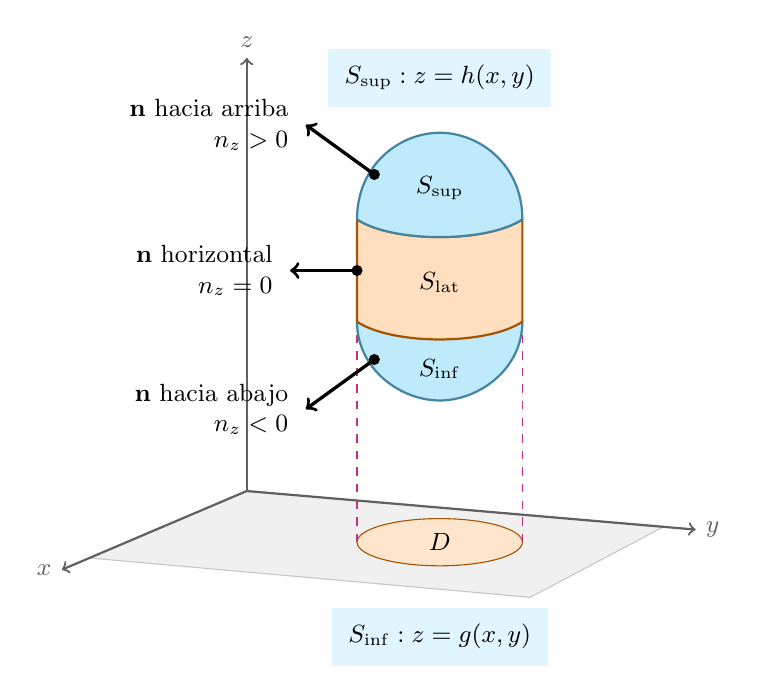
\begin{tikzpicture}[every node/.style={font=\small},line join=round]
% Plano xy y ejes en perspectiva.
\filldraw[fill=gray!12,draw=gray!45] (0,0)--(-2,-.85)--(3.6,-1.35)--(5.3,-.45)--cycle;
\draw[->,gray!75!black,thick] (0,0)--(-2.35,-1) node[left] {$x$};
\draw[->,gray!75!black,thick] (0,0)--(5.7,-.49) node[right] {$y$};
\draw[->,gray!75!black,thick] (0,0)--(0,5.5) node[above] {$z$};
% Proyecci?n y generatrices de referencia.
\filldraw[fill=orange!20,draw=orange!65!black] (2.45,-.65) ellipse (1.05 and .3);
\node at (2.45,-.65) {$D$};
\draw[magenta!75!black,dashed] (1.4,-.65)--(1.4,2.15);
\draw[magenta!75!black,dashed] (3.5,-.65)--(3.5,2.15);
% Tapa inferior, pared y tapa superior.
\filldraw[fill=cyan!25,draw=cyan!60!black,thick]
(1.4,2.15)..controls (1.4,1.55) and (1.95,1.15)..(2.45,1.15)
..controls (2.95,1.15) and (3.5,1.55)..(3.5,2.15)
..controls (3.05,2.42) and (1.85,2.42)..(1.4,2.15)--cycle;
\filldraw[fill=orange!25,draw=orange!65!black,thick]
(1.4,2.15)--(1.4,3.45)
..controls (1.85,3.15) and (3.05,3.15)..(3.5,3.45)
--(3.5,2.15)..controls (3.05,1.85) and (1.85,1.85)..(1.4,2.15)--cycle;
\filldraw[fill=cyan!25,draw=cyan!60!black,thick]
(1.4,3.45)..controls (1.4,4.15) and (1.95,4.55)..(2.45,4.55)
..controls (2.95,4.55) and (3.5,4.15)..(3.5,3.45)
..controls (3.05,3.15) and (1.85,3.15)..(1.4,3.45)--cycle;
\node at (2.45,3.85) {$S_{\rm sup}$};
\node at (2.45,2.65) {$S_{\rm lat}$};
\node at (2.45,1.55) {$S_{\rm inf}$};
% Normales y anotaciones separadas del s?lido.
\fill (1.62,4.02) circle (2pt);
\draw[->,very thick] (1.62,4.02)--(.75,4.65);
\node[anchor=east,align=right] at (.65,4.65) {$\mathbf n$ hacia arriba\\$n_z>0$};
\fill (1.4,2.8) circle (2pt);
\draw[->,very thick] (1.4,2.8)--(.55,2.8);
\node[anchor=east,align=right] at (.45,2.8) {$\mathbf n$ horizontal\\$n_z=0$};
\fill (1.62,1.67) circle (2pt);
\draw[->,very thick] (1.62,1.67)--(.75,1.04);
\node[anchor=east,align=right] at (.65,1.04) {$\mathbf n$ hacia abajo\\$n_z<0$};
\node[fill=cyan!12,inner sep=6pt] at (2.45,5.25) {$S_{\rm sup}:z=h(x,y)$};
\node[fill=cyan!12,inner sep=6pt] at (2.45,-1.85) {$S_{\rm inf}:z=g(x,y)$};
\end{tikzpicture}
\end{center}
\endgroup

En la tapa superior $z=h(x,y)$, el sólido queda debajo de la gráfica y la normal exterior apunta hacia arriba. Se tiene
\[
\mathbf n\,dS=\langle-h_x,-h_y,1\rangle\,dA.
\]
Por la fórmula del flujo sobre una gráfica, la integral doble sobre $D$ se identifica con la integral de superficie mediante
\begin{align*}
\iint_D R(x,y,h(x,y))\,dA
&=\iint_D\langle0,0,R(x,y,h(x,y))\rangle
\cdot\langle-h_x,-h_y,1\rangle\,dA\\
&=\iint_{S_{\rm sup}}\langle0,0,R\rangle\cdot\mathbf n\,dS.
\end{align*}
En la tapa inferior $z=g(x,y)$, la normal exterior apunta hacia abajo, por lo que
\[
\mathbf n\,dS=\langle g_x,g_y,-1\rangle\,dA.
\]
En consecuencia,
\begin{align*}
-\iint_D R(x,y,g(x,y))\,dA
&=\iint_D\langle0,0,R(x,y,g(x,y))\rangle
\cdot\langle g_x,g_y,-1\rangle\,dA\\
&=\iint_{S_{\rm inf}}\langle0,0,R\rangle\cdot\mathbf n\,dS.
\end{align*}

Si existe una pared lateral, esta se proyecta sobre $\partial D$. Para un arco $(x(t),y(t))$ de esa frontera, la pared se parametriza mediante $\vec r(t,z)=\langle x(t),y(t),z\rangle$, con $g(x(t),y(t))\leq z\leq h(x(t),y(t))$. Sus vectores tangentes satisfacen
\[
\vec r_t=\langle x'(t),y'(t),0\rangle,
\qquad \vec r_z=\langle0,0,1\rangle,
\qquad \vec r_t\times\vec r_z=\langle y'(t),-x'(t),0\rangle.
\]
La normal a esta pared es horizontal y, por tanto, perpendicular al campo vertical $\langle0,0,R\rangle$. Es la normal la que es ortogonal al campo; el campo es tangente a la pared. En cualquier punto regular de ella,
\[
\langle0,0,R\rangle\cdot\mathbf n
=\langle0,0,R\rangle\cdot\langle n_x,n_y,0\rangle=0,
\qquad
\iint_{S_{\rm lat}}\langle0,0,R\rangle\cdot\mathbf n\,dS=0.
\]
Al reunir las contribuciones, queda explícita la igualdad entre la integral doble y el flujo por toda la frontera:
\begin{align*}
\iiint_E R_z\,dV
&=\iint_D[R(x,y,h(x,y))-R(x,y,g(x,y))]\,dA\\
&=\iint_{S_{\rm sup}}\langle0,0,R\rangle\cdot\mathbf n\,dS
 +\iint_{S_{\rm inf}}\langle0,0,R\rangle\cdot\mathbf n\,dS\\
&\quad+\underbrace{\iint_{S_{\rm lat}}\langle0,0,R\rangle\cdot\mathbf n\,dS}_{=\,0}\\
&=\iint_{\partial E}\langle0,0,R\rangle\cdot\mathbf n\,dS
=\iint_{\partial E}R n_z\,dS.
\end{align*}
Si no hay pared lateral, solo se suman las dos tapas.

Para la componente $P$, se usa una representación elemental en $x$:
\[
E=\{(x,y,z):(y,z)\in D_x,\ a(y,z)\leq x\leq b(y,z)\}.
\]
Se denotan por $S_b$ y $S_a$ las caras $x=b(y,z)$ y $x=a(y,z)$. Sus elementos normales exteriores son, respectivamente,
\[
\mathbf n\,dS=\langle1,-b_y,-b_z\rangle\,dy\,dz,
\qquad
\mathbf n\,dS=\langle-1,a_y,a_z\rangle\,dy\,dz.
\]
Por tanto,
\begin{align*}
\iint_{D_x}P(b(y,z),y,z)\,dy\,dz
&=\iint_{S_b}\langle P,0,0\rangle\cdot\mathbf n\,dS,\\
-\iint_{D_x}P(a(y,z),y,z)\,dy\,dz
&=\iint_{S_a}\langle P,0,0\rangle\cdot\mathbf n\,dS.
\end{align*}
En las paredes laterales paralelas al eje $x$, si existen, la normal es perpendicular a ese eje. Así, $n_x=0$ y $\langle P,0,0\rangle\cdot\mathbf n=P n_x=0$. El teorema fundamental del cálculo y las igualdades anteriores dan
\begin{align*}
\iiint_E P_x\,dV
&=\iint_{D_x}[P(b(y,z),y,z)-P(a(y,z),y,z)]\,dy\,dz\\
&=\iint_{S_b}\langle P,0,0\rangle\cdot\mathbf n\,dS
 +\iint_{S_a}\langle P,0,0\rangle\cdot\mathbf n\,dS\\
&=\iint_{\partial E}\langle P,0,0\rangle\cdot\mathbf n\,dS
=\iint_{\partial E}P n_x\,dS.
\end{align*}

Para la componente $Q$, se escribe $c(x,z)\leq y\leq d(x,z)$ sobre $D_y$. Las caras $S_d$ y $S_c$ tienen elementos normales exteriores
\[
\mathbf n\,dS=\langle-d_x,1,-d_z\rangle\,dx\,dz,
\qquad
\mathbf n\,dS=\langle c_x,-1,c_z\rangle\,dx\,dz.
\]
La identificación de las integrales dobles con los flujos es
\begin{align*}
\iint_{D_y}Q(x,d(x,z),z)\,dx\,dz
&=\iint_{S_d}\langle0,Q,0\rangle\cdot\mathbf n\,dS,\\
-\iint_{D_y}Q(x,c(x,z),z)\,dx\,dz
&=\iint_{S_c}\langle0,Q,0\rangle\cdot\mathbf n\,dS.
\end{align*}
En las paredes laterales paralelas al eje $y$, si existen, la normal es perpendicular al campo $\langle0,Q,0\rangle$, de modo que $\langle0,Q,0\rangle\cdot\mathbf n=Q n_y=0$. Por ello,
\begin{align*}
\iiint_E Q_y\,dV
&=\iint_{D_y}[Q(x,d(x,z),z)-Q(x,c(x,z),z)]\,dx\,dz\\
&=\iint_{S_d}\langle0,Q,0\rangle\cdot\mathbf n\,dS
 +\iint_{S_c}\langle0,Q,0\rangle\cdot\mathbf n\,dS\\
&=\iint_{\partial E}\langle0,Q,0\rangle\cdot\mathbf n\,dS
=\iint_{\partial E}Q n_y\,dS.
\end{align*}
La suma de las tres identidades, usando $\mathbf F\cdot\mathbf n=P n_x+Q n_y+R n_z$, demuestra la fórmula en una pieza elemental en las tres direcciones.

Si $E$ se descompone en piezas $E_1,\ldots,E_m$, se aplica la identidad a cada pieza. En una cara compartida, las normales exteriores de las dos piezas son opuestas. El campo tiene el mismo valor a ambos lados, así que las dos integrales de flujo se cancelan exactamente. Las integrales triples se suman porque los interiores son disjuntos. Solo queda el flujo sobre la frontera exterior del material, incluidas las paredes de las cavidades, y se obtiene la identidad para $E$.

Cuando una representación tiene pendientes no acotadas en un borde, se recortan las piezas antes de ese borde y se aplica la identidad ya demostrada. El paso al límite es válido si convergen las integrales de volumen y las de los parches de frontera. En particular, para una esfera los parches omitidos tienen área tendiente a cero; como el campo es continuo en un entorno compacto de la esfera, está acotado y su flujo por esos parches tiende a cero. Las caras auxiliares de recorte también tienen área tendiente a cero. Esto justifica el uso de la fórmula en ese caso y completa la demostración bajo las hipótesis indicadas.
\end{proof}

En cada caso, la contribución es el valor de la componente del campo en el extremo de coordenada mayor menos su valor en el extremo de coordenada menor. Los elementos normales escritos corresponden a las caras extremas; en las paredes paralelas a la dirección de integración, la componente normal correspondiente es cero.


\begingroup\shorthandoff{>}
\begin{center}
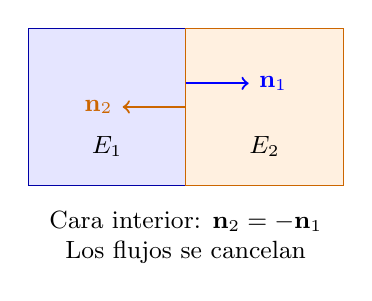
\begin{tikzpicture}[every node/.style={font=\small}]
\filldraw[fill=blue!10,draw=blue!65!black] (0,0) rectangle (2,2);
\filldraw[fill=orange!12,draw=orange!80!black] (2,0) rectangle (4,2);
\node at (1,.5) {$E_1$}; \node at (3,.5) {$E_2$};
\draw[->,thick,blue] (2,1.3)--(2.8,1.3) node[right] {$\mathbf n_1$};
\draw[->,thick,orange!80!black] (2,1)--(1.2,1) node[left] {$\mathbf n_2$};
\node[below,align=center] at (2,-.2) {Cara interior: $\mathbf n_2=-\mathbf n_1$\\Los flujos se cancelan};
\end{tikzpicture}
\end{center}
\endgroup

\paragraph{Ejemplo 1. Campo radial en una esfera}
Se desea calcular el flujo por la esfera $\partial E$ con orientación exterior. El campo es polinómico, por lo que sus derivadas parciales son continuas en todo $\mathbb R^3$. Su divergencia es
\[
\nabla\cdot\mathbf F
=\frac{\partial x}{\partial x}+\frac{\partial y}{\partial y}
+\frac{\partial z}{\partial z}=1+1+1=3.
\]
Por Gauss, el flujo se convierte en una integral sobre la bola:
\[
\Phi_{\partial E}=\iiint_E3\,dV=3\operatorname{vol}(E).
\]
También se puede comprobar el resultado directamente sobre la superficie. El vector $\langle x,y,z\rangle$ apunta desde el centro hacia la esfera y tiene longitud $a$ en ella. Por tanto, la normal unitaria exterior y el producto punto son
\[
\mathbf n=\frac{\langle x,y,z\rangle}{a},
\qquad
\mathbf F\cdot\mathbf n=\frac{x^2+y^2+z^2}{a}
=\frac{a^2}{a}=a.
\]
Como este valor es constante sobre la esfera de área $4\pi a^2$,
\[
\iint_{\partial E}\mathbf F\cdot\mathbf n\,dS
=a\iint_{\partial E}dS=a(4\pi a^2)=4\pi a^3.
\]
El flujo es positivo y el campo sale por toda la frontera: en cada punto se cumple $\mathbf F=a\mathbf n$, como muestra la figura.

\begingroup\shorthandoff{>}
\begin{center}
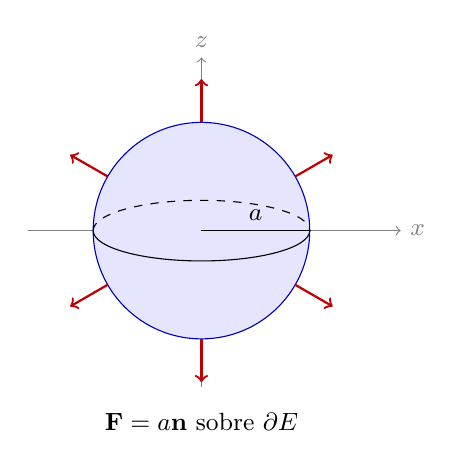
\begin{tikzpicture}[scale=1.1,every node/.style={font=\small}]
\draw[->,gray] (-2,0)--(2.3,0) node[right] {$x$};
\draw[->,gray] (0,-1.8)--(0,2) node[above] {$z$};
\filldraw[fill=blue!10,draw=blue!70!black] (0,0) circle (1.25);
\draw[dashed] (-1.25,0) arc (180:0:1.25 and .35);
\draw (-1.25,0) arc (180:360:1.25 and .35);
\foreach \t in {30,90,150,210,270,330}
\draw[->,red!75!black,thick] ({1.25*cos(\t)},{1.25*sin(\t)})--({1.75*cos(\t)},{1.75*sin(\t)});
\draw (0,0)--(1.25,0) node[midway,above] {$a$};
\node[below] at (0,-2) {$\mathbf F=a\mathbf n$ sobre $\partial E$};
\end{tikzpicture}
\end{center}
\endgroup

\paragraph{Ejemplo 2. Transporte uniforme por una caja}
Sea $E=[0,a]\times[0,b]\times[0,c]$, con $a,b,c>0$, y sea $\mathbf F=\langle u,0,0\rangle$, donde $u>0$ es constante. Se calcula el flujo exterior por las seis caras de la caja. El campo apunta en la dirección positiva del eje $x$ y tiene la misma magnitud en todos los puntos.

Como todas sus componentes son constantes, se tiene
\[
\nabla\cdot\mathbf F
=\frac{\partial u}{\partial x}+\frac{\partial0}{\partial y}
+\frac{\partial0}{\partial z}=0.
\]
El campo es de clase $C^1$ en todo el espacio, y la caja tiene frontera cerrada y suave por partes. Por el teorema de Gauss,
\[
\Phi_{\partial E}=\iiint_E0\,dV=0.
\]
Para interpretar este resultado, se calculan las contribuciones de las caras. En $x=0$, la normal exterior es $\langle-1,0,0\rangle$, porque el exterior se encuentra hacia los valores negativos de $x$. En $x=a$, la normal es $\langle1,0,0\rangle$. Ambas caras son rect?ngulos de lados $b$ y $c$, y en ellas $dS=dy\,dz$. Por tanto,
\begin{align*}
\Phi_{x=0}
&=\int_0^c\int_0^b
\langle u,0,0\rangle\cdot\langle-1,0,0\rangle\,dy\,dz
=\int_0^c\int_0^b(-u)\,dy\,dz=-ubc,\\
\Phi_{x=a}
&=\int_0^c\int_0^b
\langle u,0,0\rangle\cdot\langle1,0,0\rangle\,dy\,dz
=\int_0^c\int_0^b u\,dy\,dz=ubc.
\end{align*}
En las caras $y=0$ y $y=b$, las normales son $\langle0,-1,0\rangle$ y $\langle0,1,0\rangle$. En las caras $z=0$ y $z=c$, son $\langle0,0,-1\rangle$ y $\langle0,0,1\rangle$. Todas son perpendiculares a $\mathbf F$, de modo que el producto punto es cero en cada una de esas cuatro caras. Al sumar,
\[
\Phi_{\partial E}=\Phi_{x=0}+\Phi_{x=a}
+\Phi_{y=0}+\Phi_{y=b}+\Phi_{z=0}+\Phi_{z=c}
=-ubc+ubc=0.
\]
El signo negativo en $x=0$ representa entrada y el positivo en $x=a$ representa salida. Si $\mathbf F$ es una velocidad, entran y salen $ubc$ unidades de volumen por unidad de tiempo. Así, el flujo neto nulo expresa un balance entre entrada y salida, aunque hay transporte a través de la caja.

\begingroup\shorthandoff{>}
\begin{center}
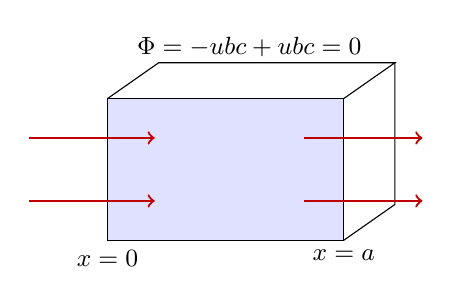
\begin{tikzpicture}[x={(1cm,0cm)},y={(.5cm,.35cm)},z={(0cm,1cm)},every node/.style={font=\small}]
\filldraw[fill=blue!12] (0,0,0)--(3,0,0)--(3,0,1.8)--(0,0,1.8)--cycle;
\draw (0,0,1.8)--(0,1.3,1.8)--(3,1.3,1.8)--(3,0,1.8);
\draw (3,0,0)--(3,1.3,0)--(3,1.3,1.8);
\foreach \h in {.5,1.3} {
\draw[->,red!75!black,thick] (-1,0,\h)--(.6,0,\h);
\draw[->,red!75!black,thick] (2.5,0,\h)--(4,0,\h);}
\node[below] at (0,0,0) {$x=0$}; \node[below] at (3,0,0) {$x=a$};
\node[above] at (1.5,.6,2) {$\Phi=-ubc+ubc=0$};
\end{tikzpicture}
\end{center}
\endgroup

\paragraph{Ejemplo 3. Un sólido con cavidad}
Sea $E:a\leq\sqrt{x^2+y^2+z^2}\leq b$, donde $0<a<b$, y sea $\mathbf F=\langle x,y,z\rangle$. El sólido es una corona esférica: contiene el material entre los radios $a$ y $b$, pero excluye la bola de radio $a$. Su frontera tiene dos componentes,
\[
S_b:x^2+y^2+z^2=b^2,\qquad
S_a:x^2+y^2+z^2=a^2,\qquad
\partial E=S_b\cup S_a.
\]
El campo es suave en todo el espacio y su divergencia es $1+1+1=3$. Gauss se aplica al material de la corona, de modo que
\[
\Phi_{\partial E}=\iiint_E3\,dV.
\]
Esta integral equivale a tres veces el volumen del material,
\[
\operatorname{vol}(E)=\frac{4\pi b^3}{3}-\frac{4\pi a^3}{3}.
\]
Para comprobar la orientaci?n de cada componente, se calculan sus flujos por separado. En $S_b$, salir del material significa alejarse del origen, as? que
\[
\mathbf n_b=\frac{\langle x,y,z\rangle}{b},
\qquad \mathbf F\cdot\mathbf n_b
=\frac{x^2+y^2+z^2}{b}=b.
\]
En consecuencia,
\[
\Phi_{S_b}=\iint_{S_b}b\,dS=b(4\pi b^2)=4\pi b^3.
\]
En $S_a$, salir del material significa entrar en la cavidad, es decir, dirigirse hacia el origen. La normal exterior a $E$ en esta superficie es
\[
\mathbf n_a=-\frac{\langle x,y,z\rangle}{a},
\qquad \mathbf F\cdot\mathbf n_a
=-\frac{x^2+y^2+z^2}{a}=-a.
\]
Por tanto,
\[
\Phi_{S_a}=\iint_{S_a}(-a)\,dS=-a(4\pi a^2)=-4\pi a^3.
\]
El flujo por toda la frontera es la suma de ambas contribuciones:
\[
\Phi_{\partial E}=\Phi_{S_b}+\Phi_{S_a}
=4\pi b^3-4\pi a^3,
\]
que coincide con la integral triple. El campo entra en el material a través de la esfera interior y sale a través de la exterior. El signo negativo de la contribución interior se debe a la normal elegida respecto al material, como muestra la sección de la figura.

\begingroup\shorthandoff{>}
\begin{center}
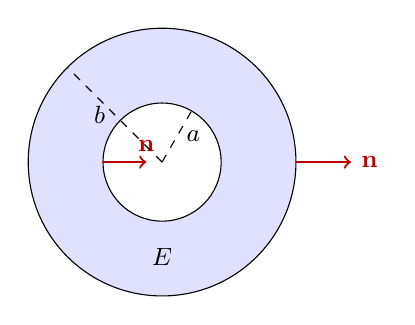
\begin{tikzpicture}[every node/.style={font=\small}]
\fill[blue!12,even odd rule] (0,0) circle (1.7) (0,0) circle (.75);
\draw (0,0) circle (1.7); \draw (0,0) circle (.75);
\draw[->,red!75!black,thick] (1.7,0)--(2.4,0) node[right] {$\mathbf n$};
\draw[->,red!75!black,thick] (-.75,0)--(-.2,0) node[above] {$\mathbf n$};
\draw[dashed] (0,0)--({.75*cos(60)},{.75*sin(60)}) node[midway,right] {$a$};
\draw[dashed] (0,0)--({1.7*cos(135)},{1.7*sin(135)}) node[midway,left] {$b$};
\node at (0,-1.2) {$E$};
\end{tikzpicture}
\end{center}
\endgroup

\subsection{Interpretación geométrica y física}

Para $\mathbf F=\langle x,y,z\rangle$ la divergencia es $3$: cada volumen tiene flujo neto saliente. Para $\mathbf F=-\langle x,y,z\rangle$ vale $-3$: predomina la entrada. Para $\mathbf F=\langle1,0,0\rangle$ vale cero: lo que entra se compensa con lo que sale. Los diagramas muestran secciones en el plano $xz$ de pequeñas bolas centradas en el origen; las flechas representan el campo.

\begingroup\shorthandoff{>}
\begin{center}
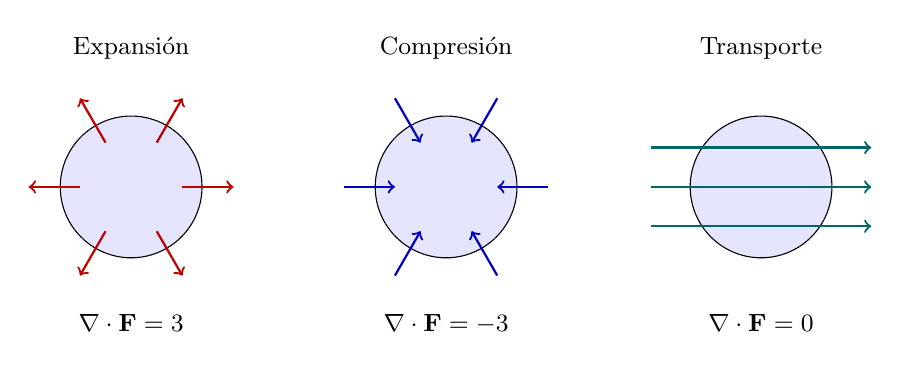
\begin{tikzpicture}[every node/.style={font=\small}]
\foreach \s/\titulo in {0/Expansión,4/Compresión,8/Transporte} {
\begin{scope}[shift={(\s,0)}]
\filldraw[fill=blue!10] (0,0) circle (.9);
\node[above] at (0,1.5) {\titulo};
\end{scope}}
\foreach \t in {0,60,120,180,240,300} {
\draw[->,red!75!black,thick] ({.65*cos(\t)},{.65*sin(\t)})--({1.3*cos(\t)},{1.3*sin(\t)});
\draw[->,blue!75!black,thick] ({4+1.3*cos(\t)},{1.3*sin(\t)})--({4+.65*cos(\t)},{.65*sin(\t)});}
\foreach \h in {-.5,0,.5} \draw[->,teal!80!black,thick] (6.6,\h)--(9.4,\h);
\node[below] at (0,-1.5) {$\nabla\cdot\mathbf F=3$};
\node[below] at (4,-1.5) {$\nabla\cdot\mathbf F=-3$};
\node[below] at (8,-1.5) {$\nabla\cdot\mathbf F=0$};
\end{tikzpicture}
\end{center}
\endgroup

\begingroup\shorthandoff{>}
\begin{center}
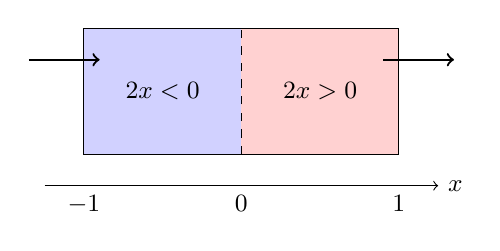
\begin{tikzpicture}[every node/.style={font=\small}]
\fill[blue!18] (-2,0) rectangle (0,1.6);
\fill[red!18] (0,0) rectangle (2,1.6);
\draw (-2,0) rectangle (2,1.6); \draw[dashed] (0,0)--(0,1.6);
\node at (-1,.8) {$2x<0$}; \node at (1,.8) {$2x>0$};
\draw[->] (-2.5,-.4)--(2.5,-.4) node[right] {$x$};
\node[below] at (-2,-.4) {$-1$}; \node[below] at (0,-.4) {$0$}; \node[below] at (2,-.4) {$1$};
\draw[->,thick] (-2.7,1.2)--(-1.8,1.2);
\draw[->,thick] (1.8,1.2)--(2.7,1.2);
\end{tikzpicture}
\end{center}
\endgroup

\begin{mynote}{Un campo singular}
El campo $\mathbf F=\langle x,y,z\rangle/(x^2+y^2+z^2)^{3/2}$ tiene divergencia cero fuera del origen. Sin embargo, en una esfera de radio $a$ su componente normal exterior es $1/a^2$, de modo que el flujo es $4\pi$. No se puede aplicar Gauss a la bola porque el campo no está definido en el origen. En una corona esférica que excluye el origen sí se puede aplicar: el flujo exterior $4\pi$ se compensa con el flujo $-4\pi$ de la frontera interior.
\end{mynote}

\paragraph{Ejemplo 4. Flujo por la frontera de un cilindro}
Sea $E:x^2+y^2\leq a^2$, $0\leq z\leq L$, con $a,L>0$, y sea $\mathbf F=\langle xz,yz,z^2\rangle$. El campo es polinómico y la frontera incluye la pared y las dos tapas. Como
\[
\nabla\cdot\mathbf F=z+z+2z=4z,
\]
las coordenadas cilíndricas dan
\begin{align*}
\Phi_{\partial E}
&=\int_0^{2\pi}\int_0^a\int_0^L4z\,r\,dz\,dr\,d\theta\\
&=\int_0^{2\pi}\int_0^a2L^2r\,dr\,d\theta
=2\pi a^2L^2.
\end{align*}
En la tapa inferior el campo es cero; en la superior, $\mathbf n=\langle0,0,1\rangle$, de modo que el flujo es $\pi a^2L^2$. Por tanto, la pared lateral aporta el flujo restante $\pi a^2L^2$.

\begingroup\shorthandoff{>}
\begin{center}
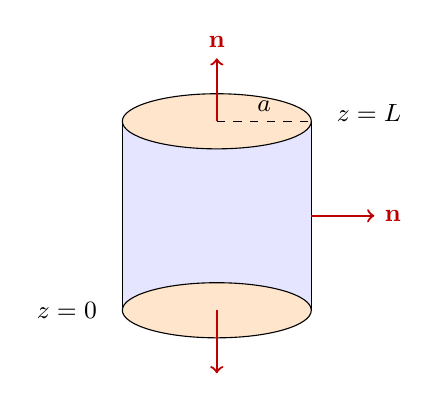
\begin{tikzpicture}[every node/.style={font=\small}]
\fill[blue!10] (-1.2,0) rectangle (1.2,2.4);
\draw (-1.2,0)--(-1.2,2.4); \draw (1.2,0)--(1.2,2.4);
\draw[fill=orange!20] (0,2.4) ellipse (1.2 and .35);
\filldraw[fill=orange!20,draw=black] (0,0) ellipse (1.2 and .35);
\draw[->,red!75!black,thick] (0,2.4)--(0,3.2) node[above] {$\mathbf n$};
\draw[->,red!75!black,thick] (1.2,1.2)--(2,1.2) node[right] {$\mathbf n$};
\draw[->,red!75!black,thick] (0,0)--(0,-.8);
\node[right] at (1.4,2.5) {$z=L$};
\node[left] at (-1.4,0) {$z=0$};
\draw[dashed] (0,2.4)--(1.2,2.4) node[midway,above] {$a$};
\end{tikzpicture}
\end{center}
\endgroup

\paragraph{Ejemplo 5. Flujo exterior por un paraboloide abierto}
Sea $S:z=4-x^2-y^2$, $z\geq0$, orientada hacia arriba, y sea $\mathbf F=\langle x,y,z+1\rangle$. Se cierra $S$ con el disco $B:z=0$, $x^2+y^2\leq4$. El sólido es
\[
E=\{(x,y,z):x^2+y^2\leq4,\ 0\leq z\leq4-x^2-y^2\}.
\]
La orientación hacia arriba en $S$ es exterior a $E$, mientras que en $B$ la normal exterior es $\langle0,0,-1\rangle$. La divergencia vale $3$, y
\begin{align*}
\Phi_S+\Phi_B
&=3\int_0^{2\pi}\int_0^2\int_0^{4-r^2}r\,dz\,dr\,d\theta\\
&=6\pi\int_0^2(4r-r^3)\,dr
=24\pi.
\end{align*}
En el disco, $\mathbf F\cdot\mathbf n=-1$, así que $\Phi_B=-4\pi$. En consecuencia,
\[
\Phi_S=24\pi-(-4\pi)=28\pi.
\]
La base añadida tiene flujo entrante; por ello, el flujo saliente por el paraboloide supera al flujo neto de la superficie cerrada.

\begingroup\shorthandoff{>}
\begin{center}
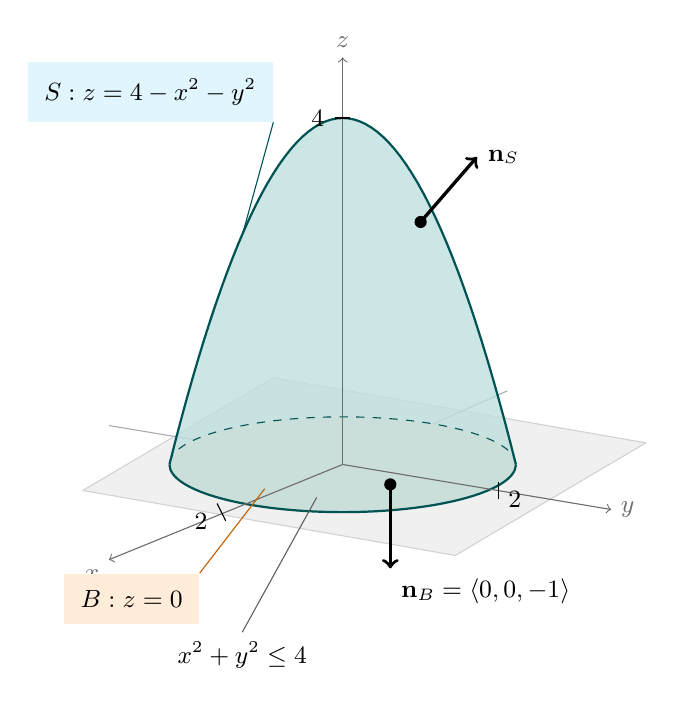
\begin{tikzpicture}[scale=1.1,every node/.style={font=\small},line join=round]
% Plano de cierre, representado en perspectiva.
\filldraw[fill=gray!12,draw=gray!35]
(-3,-.3)--(-.8,1)--(3.5,.25)--(1.3,-1.05)--cycle;
\draw[gray!65] (0,0)--(1.9,.85);
\draw[gray!65] (0,0)--(-2.7,.45);
% El disco se rellena antes de dibujar la superficie.
\fill[orange!22] (0,0) ellipse (2 and .55);
% Perfil del paraboloide y borde del disco.
\path[fill=teal!25,fill opacity=.8]
plot[domain=-2:2,samples=61] (\x,{4-\x*\x})
arc[start angle=0,end angle=-180,x radius=2,y radius=.55]--cycle;
\draw[teal!65!black,thick]
plot[domain=-2:2,samples=61] (\x,{4-\x*\x});
\draw[teal!65!black,dashed] (2,0)
arc[start angle=0,end angle=180,x radius=2,y radius=.55];
\draw[teal!65!black,thick] (-2,0)
arc[start angle=180,end angle=360,x radius=2,y radius=.55];
% Ejes y marcas de referencia.
\draw[->,gray!85!black] (0,0)--(-2.7,-1.1) node[below left] {$x$};
\draw[->,gray!85!black] (0,0)--(3.1,-.52) node[right] {$y$};
\draw[->,gray!85!black] (0,0)--(0,4.7) node[above] {$z$};
\draw (-.09,4)--(.09,4) node[left,xshift=-6pt] {$4$};
\draw (-1.35,-.65)--(-1.45,-.45) node[below left] {$2$};
\draw (1.8,-.4)--(1.8,-.2) node[below right] {$2$};
% Normales exteriores: ascendente en S y descendente en B.
\fill (.9,2.8) circle (2pt);
\draw[->,very thick] (.9,2.8)--(1.55,3.55)
node[right] {$\mathbf n_S$};
\fill (.55,-.23) circle (2pt);
\draw[->,very thick] (.55,-.23)--(.55,-1.2)
node[below right] {$\mathbf n_B=\langle0,0,-1\rangle$};
% Etiquetas separadas del s?lido.
\node[fill=cyan!12,inner sep=6pt,anchor=east] (sup) at (-.8,4.3)
{$S:z=4-x^2-y^2$};
\draw[teal!65!black] (sup.south east)--(-1.15,2.68);
\node[fill=orange!15,inner sep=6pt,anchor=east] (base) at (-1.65,-1.55)
{$B:z=0$};
\draw[orange!75!black] (base.north east)--(-.9,-.28);
\node[anchor=east] (dom) at (-.3,-2.2) {$x^2+y^2\leq4$};
\draw[gray!75!black] (dom.north)--(-.3,-.38);
\end{tikzpicture}
\end{center}
\endgroup

\subsection{Ejercicios}
En todos los problemas de flujo por una superficie cerrada se adopta la orientación exterior, salvo que se indique otra.
\begin{enumerate}
    \setlength{\itemsep}{1pt}
    \item Determine la divergencia de los campos $\langle x^2,yz,z^2\rangle$, $\langle-y,x,0\rangle$ y $\langle e^x,\sin y,\cos z\rangle$. Indique sus dominios.

    \item Determine si se puede aplicar el teorema de Gauss al campo $\mathbf F=\langle x,y,z\rangle/(x^2+y^2+z^2)^{3/2}$ en cada sólido: la bola de radio $1$ centrada en el origen, la corona $1\leq\sqrt{x^2+y^2+z^2}\leq2$ y la bola de radio $1$ centrada en $(3,0,0)$. Justifique.

    \item Calcule el flujo de $\mathbf F=\langle2x,-y,3z\rangle$ por la frontera de $[0,1]\times[0,2]\times[0,3]$ mediante el teorema de la divergencia.

    \item Calcule el flujo de $\mathbf F=\langle x,y,z\rangle$ por la esfera de radio $a>0$ centrada en el origen con orientación interior.

    \item Calcule el flujo de $\mathbf F=\langle x^2,y^2,z^2\rangle$ por la frontera del tetraedro $x,y,z\geq0$, $x+y+z\leq1$.

    \item Calcule el flujo de $\mathbf F=\langle x^3,y^3,z^3\rangle$ por la esfera $x^2+y^2+z^2=a^2$, con $a>0$.

    \item Calcule el flujo de $\mathbf F=\langle xz,yz,z^2\rangle$ por la frontera del sólido $x^2+y^2\leq z\leq4$.

    \item Calcule el flujo de $\mathbf F=\langle x,y,z\rangle$ por la superficie lateral del cono $z=\sqrt{x^2+y^2}$, $0\leq z\leq h$, con $h>0$, orientada hacia afuera del sólido $\sqrt{x^2+y^2}\leq z\leq h$.

    \item Calcule el flujo de $\mathbf F=\langle x,y,z+2\rangle$ por el hemisferio $x^2+y^2+z^2=9$, $z\geq0$, con orientación radial exterior.

    \item El flujo eléctrico de un campo eléctrico $\mathbf E$ a través de una superficie orientada $S$ se define por
\[
\Phi_{\rm e}=\iint_S\mathbf E\cdot\mathbf n\,dS,
\]
donde $\mathbf n$ es la normal unitaria elegida. Una esfera maciza de radio $R>0$, centrada en el origen, tiene carga distribuida uniformemente con densidad volumétrica $\rho_0$ (carga por unidad de volumen). En su interior, el campo está dado por
\[
\mathbf E(x,y,z)=\frac{\rho_0}{3\varepsilon_0}\langle x,y,z\rangle,
\qquad x^2+y^2+z^2<R^2,
\]
donde $\varepsilon_0>0$ es la permitividad eléctrica del vacío, una constante que relaciona la carga con el campo eléctrico. Para $0<a<R$, calcule mediante el teorema de la divergencia el flujo eléctrico exterior por $S_a:x^2+y^2+z^2=a^2$.
    \item Sea $E$ un sólido con frontera $S=\partial E$ y normal unitaria exterior $\mathbf n$, que satisface las hipótesis geométricas del teorema de la divergencia. Sean $f$ y $g$ funciones de clase $C^2$ en un abierto que contiene a $E$. Se definen el laplaciano y la derivada normal por
\[
\nabla^2 g=g_{xx}+g_{yy}+g_{zz},
\qquad D_{\mathbf n}g=\nabla g\cdot\mathbf n.
\]
Demuestre la identidad
\[
\iiint_E\bigl(f\nabla^2g+\nabla f\cdot\nabla g\bigr)\,dV
=\iint_S fD_{\mathbf n}g\,dS.
\]
(hint: Utilice la regla del producto $\nabla\cdot(f\mathbf G)=f\nabla\cdot\mathbf G+\nabla f\cdot\mathbf G$.)

    \item Bajo las mismas hipótesis y con la notación del ejercicio anterior, defina $\nabla^2f=f_{xx}+f_{yy}+f_{zz}$ y $D_{\mathbf n}f=\nabla f\cdot\mathbf n$. Demuestre la identidad
\[
\iiint_E\bigl(f\nabla^2g-g\nabla^2f\bigr)\,dV
=\iint_S\bigl(fD_{\mathbf n}g-gD_{\mathbf n}f\bigr)\,dS.
\]
(hint: Utilice el ejercicio anterior dos veces, intercambiando $f$ y $g$.)

\end{enumerate}
